
\subsection{圆锥}
\begin{frame}
    \frametitle{圆锥知识点}
    \begin{itemize}
        \item 圆锥母线长公式:\( l = \sqrt{r^2 + h^2} \)
        \item 圆锥侧面积公式:\( S_{\text{侧}} = \pi r l \)
        \item 圆锥表面积公式:\( S_{\text{表}} = \pi r(r + l) \)
        \item 圆锥体积公式:\( V = \frac{1}{3}\pi r^2 h \)
    \end{itemize}
    
    \vspace{0.5cm}
    
    \begin{columns}
        \column{0.5\textwidth}
        \begin{block}{符号说明}
            \begin{itemize}
                \item \( r \): 底面半径
                \item \( h \): 高
                \item \( l \): 母线长
            \end{itemize}
        \end{block}
        
        \column{0.5\textwidth}
        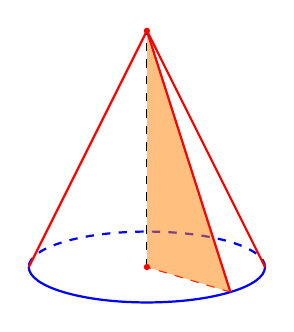
\begin{tikzpicture}[scale=1.5,
            y={(0cm,-0.3cm)}, % 设置 x 轴方向
            x={(1cm,0cm)},            % 设置 y 轴方向
            z={(0cm,1cm)}             % 设置 z 轴方向
        ]
            % 定义圆柱的参数
            \def\radius{1} % 圆锥底面半径
            \def\height{2} % 圆锥的高度
            % 一些坐标
            \coordinate (O') at (0,0,\height);
            \coordinate (O) at (0,0,0);
            %上圆上一点
            \coordinate (A') at ({\radius*sqrt(2)/2},{\radius*sqrt(2)/2},\height);
            %下圆上一点
            \coordinate (A) at ({\radius*sqrt(2)/2},{\radius*sqrt(2)/2},0);
                % 底面半径
                \draw[thin,dashed,red] (A) -- (O);
                % 绘制底面圆
                \begin{scope}
                    \draw [blue,thick,dashed] (\radius,0,0) arc (0:-180:\radius) ;
                    \draw [blue,thick] (\radius,0,0) arc (0:180:\radius) ;
        
                \end{scope}
                \fill[orange,opacity=0.5] (A) -- (O) -- (O') -- cycle;
                % 绘制母线
                \begin{scope}
                    \draw[thick,red] (\radius,0,0) -- (O');
                    \draw[thick,red] (-\radius,0,0) -- (O');
                    \draw[thick,red] (A) -- (O');
                \end{scope}
                
        
                % 绘制高线
                \begin{scope}
                    \draw[thin,dashed] (0,0,0) -- (0,0,\height);
                    \fill[red] (0,0,0) circle (0.75pt);  % 绘制一个点测试一下 
                    \fill[red] (0,0,\height) circle (0.75pt);  % 绘制一个点测试一下 
                \end{scope}
        \end{tikzpicture}
    \end{columns}
\end{frame}



% 幻灯片1:题目1
\begin{frame}
    \frametitle{基础计算题 - 题目1}
    \begin{block}{题目}
        圆锥底面半径为4cm,高为3cm,求其侧面积、表面积和体积。
    \end{block}
    \pause
    
    \begin{block}{解析}
        1. 计算母线长:
        \[
        l = \sqrt{r^2 + h^2} = \sqrt{4^2 + 3^2} = 5 \, \text{cm}
        \]
        2. 
        \(
        S_{\text{侧}} = \pi r l = \pi \times 4 \times 5 = 20\pi \, \text{cm}^2
        \)\\
        3. 
        \(
        S_{\text{表}} = S_{\text{侧}} + \pi r^2 = 20\pi + \pi \times 4^2 = 36\pi \, \text{cm}^2
        \)\\
        4. 体积公式:
        \[
        V = \frac{1}{3} \pi r^2 h = \frac{1}{3} \pi \times 4^2 \times 3 = 16\pi \, \text{cm}^3
        \]
    \end{block}
    
    \begin{alertblock}{\small 答案}
        \small
        侧面积:\(20\pi \, \text{cm}^2\),表面积:\(36\pi \, \text{cm}^2\),体积:\(16\pi \, \text{cm}^3\)
    \end{alertblock}
\end{frame}

% 幻灯片2:题目2
\begin{frame}
    \frametitle{基础计算题 - 题目2}
    \begin{block}{题目}
        圆锥底面直径为6dm,母线长为8dm,求其表面积。
    \end{block}
    \pause
    
    \begin{block}{解析}
        1. 计算底面半径:
        \[
        r = \frac{d}{2} = \frac{6}{2} = 3 \, \text{dm}
        \]
        2. 侧面积公式:
        \(
        S_{\text{侧}} = \pi r l = \pi \times 3 \times 8 = 24\pi \, \text{dm}^2
        \)\\
        3. 底面积公式:
        \(
        S_{\text{底}} = \pi r^2 = \pi \times 3^2 = 9\pi \, \text{dm}^2
        \)\\
        4. 表面积公式:
        \(
        S_{\text{表}} = S_{\text{侧}} + S_{\text{底}} = 24\pi + 9\pi = 33\pi \, \text{dm}^2
        \)
    \end{block}
    
    \begin{alertblock}{答案}
        表面积:\(33\pi \, \text{dm}^2\)
    \end{alertblock}
\end{frame}

% 幻灯片3:题目3
\begin{frame}
    \frametitle{基础计算题 - 题目3}
    \begin{block}{题目}
        圆锥底面周长为\(10\pi\)m,体积为\(\frac{25}{3}\pi\)m³,求其高。
    \end{block}
    \pause
    
    \begin{block}{解析}
        1. 计算底面半径:
        \[
        C = 2\pi r \implies r = \frac{C}{2\pi} = \frac{10\pi}{2\pi} = 5 \, \text{m}
        \]
        2. 体积公式:
        \[
        V = \frac{1}{3} \pi r^2 h \implies \frac{25}{3}\pi = \frac{1}{3} \pi \times 5^2 \times h
        \]
        3. 解方程:
        \[
        \frac{25}{3}\pi = \frac{25}{3}\pi h \implies h = 1 \, \text{m}
        \]
    \end{block}
    
    \begin{alertblock}{答案}
        高:\(1 \, \text{m}\)
    \end{alertblock}
\end{frame}


\begin{frame}
    \frametitle{圆锥表面积计算- 题目4}
    
    \begin{block}{题目}
        一个圆锥的底面半径为 \(6 \, \text{cm}\),高为 \(8 \, \text{cm}\),求它的表面积(结果保留 \(\pi\))。
    \end{block}
    

\end{frame}
\begin{frame}

    \begin{block}{解析}
        \begin{enumerate}
            \item 计算母线长 \( l \):
            \[
            l = \sqrt{r^2 + h^2} = \sqrt{6^2 + 8^2} = \sqrt{100} = 10 \, \text{cm}
            \]
            
            \item 计算侧面积 \( S_{\text{侧}} \):
            \[
            S_{\text{侧}} = \pi r l = \pi \times 6 \times 10 = 60\pi \, \text{cm}^2
            \]
            
            \item 计算底面积 \( S_{\text{底}} \):
            \[
            S_{\text{底}} = \pi r^2 = \pi \times 6^2 = 36\pi \, \text{cm}^2
            \]
            
            \item 计算表面积 \( S_{\text{表}} \):
            \[
            S_{\text{表}} = S_{\text{侧}} + S_{\text{底}} = 60\pi + 36\pi = 96\pi \, \text{cm}^2
            \]
        \end{enumerate}
    \end{block}

    \begin{alertblock}{答案}
        圆锥的表面积为 \(\boxed{96\pi \, \text{cm}^2}\)。
    \end{alertblock}
\end{frame}



% 题目5
\begin{frame}{展开图相关(题目5)}
    \begin{block}{题目}
    圆锥侧面展开图是圆心角216°的扇形,底面半径5cm,求侧面积。
    \end{block}
    \pause
    
    \begin{align*}
    \text{底面周长} &= 2\pi r = 10\pi \\
    \text{扇形弧长} &= \frac{216^\circ}{360^\circ} \times 2\pi l = 10\pi \\
    \Rightarrow l &= \frac{10\pi \times 180^\circ}{216^\circ \pi} = \frac{125}{3}\text{cm} \\
    S_{\text{侧}} &= \pi r l = \pi \times 5 \times \frac{25}{3} = \frac{125}{3}\pi \,\text{cm}^2
    \end{align*}

    \end{frame}



% 题目6
\begin{frame}{展开图相关(题目6)}
    \begin{block}{题目}
    圆锥侧面展开图是半圆形,母线长10cm,求侧面积。
    \end{block}
    
    \pause

    \begin{equation*}
    \begin{cases}
    \text{半圆周长} = \pi l = 10\pi \\
    \text{底面周长} = 2\pi r = 10\pi \Rightarrow r = 5\text{cm} \\
    S_{\text{侧}} = \pi r l = \pi \times 5 \times 10 = 50\pi \,\text{cm}^2
    \end{cases}
    \end{equation*}
    \end{frame}



    % 题目7
\begin{frame}{逆向计算参数(题目7)}
    \begin{block}{题目}
    侧面积30$\pi$ cm²,底面半径4cm,求母线长。
    \end{block}
    \pause
    
    \begin{align*}
    S_{\text{侧}} &= \pi r l \\
    30\pi &= \pi \times 4 \times l \\
    l &= \frac{30\pi}{4\pi} = \frac{15}{2}\,\text{cm} \\
    \end{align*}
    

    \end{frame}
    
    % 题目8
    \begin{frame}{逆向计算参数(题目8)}
    \begin{block}{题目}
    侧面积80$\pi$ cm²,母线长10cm,求底面半径。
    \end{block}
    \pause
    
    $$
    \begin{aligned}
    S_{\text{侧}} &= \pi r l \\
    80\pi &= \pi \times r \times 10 \\
    r &= \frac{80\pi}{10\pi} = 8\text{cm}
    \end{aligned}
    $$
    
   
    \end{frame}